\chapter{Fundamentals and Related Work}
\label{chap:fundamentals}
This chapter provides the fundamental concepts and related work that are required to understand the approach to be discussed in following Chapter \ref{chap:approach}. The first section introduces definitions of terms that are used throughout this document. The second section provides a brief introduction about the basic concepts of this thesis work.  The third and fourth sections present description about  works related to the presented approach. The last section focuses on concepts of Resource-centric Organizational Modeling and its notations. Though modeling notations are not part of implementation, it has been introduced to assist the reader in better understanding. The last section also discusses about the process and entity representation of the organizational modeling.  

%%%%%%%%%%%%%%%%%%%%%%%%%%%%%%%%%%%%%%%%%%%%%%%%%%%%%%%%%%%%%%%%%%%%%%%%%
\section{Definitions of Terms}
\label{sec:termdefinitions}
%%%%%%%%%%%%%%%%%%%%%%%%%%%%%%%%%%%%%%%%%%%%%%%%%%%%%%%%%%%%%%%%%%%%%%%%%
In this section, the definitions of terminologies that are used throughout this document has been provided.

\textit{Business Process} -  A business process has been defined as the set of activities and tasks whose final output is accomplishment of a goal. These activities are performed in an organizational and technical environment \cite{Weske2012}.  Based on the type of input and the operation of tasks, these processes can be categorized as management process, support process, research process, development process, etc., \cite{Sungur2015}.   

\textit{Business Logic} - Business logic refers to the activities that need to be done to execute the corresponding process. 

\textit{Business Process Models} - Business process models are models to capture recurring procedures during a business process execution and enact them in a automated fashion for re-using those stored knowledge. A model can be in any form of representation such as graphical, descriptive etc. In our context, model refers to descriptive information of a process or an entity. 

\textit{Business Process Model and Notation (BPMN)} - BPMN is the standard notation used for business process modeling \cite{Recker2010} and business experts model their business processes mostly using BPMN \cite{SAP2009}. Models developed using BPMN can also be executed using BPMN engines. BPMN bridges the gap between developers and business experts. BPMN uses graphical representation to model the business processes.   

\textit{Business Process Engines} - Business process engines can enact the business process models automatically once the configuration of necessary infrastructure has been carried out. Also in the research article \cite{Leymann2010}, it has been mentioned that BPMN users wanted to execute the models with BPMN2.0 engine due to its operational semantics.

\textit{Business Process Management} - Business process management (BPM) includes concepts, methods, and techniques to support the design, administration, configuration, enactment, and analysis of business processes \cite{Weske2012}.

\textit{Business Process Management Life Cycle} - Business process management life cycle is the series of phases such as modeling, configuring, executing, and improving business process. These series phases are conducted as a cycle \cite{Weske2012}.

\textit{Informal Process} - The processes that human participate and create knowledge are called unstructured/informal/human-centric processes. In informal process, execution steps cannot be modeled or are not feasible to model before their enactments. This is because due to the dynamic changing behavior of execution steps of the informal processes.  For Example, software development process is an informal process, where required activities and order of their execution cannot be determined beforehand \cite{Sungur2015}. The four characteristic properties are: implicit business logic, varying relationships among resources, resource participation in multiple informal processes and changing resources \cite{Sungur2014a}.    

\textit{Informal Process Essentials} - Informal Process Essentials (IPE) is an intention-based approach that enables describing process declartively, i.e., without describing how the intention is achieved, and providing only information about what has to be achieved \cite{Sungur2014a}. 

\textit{OASIS Topology and Orchestration Specification for Cloud Applications}(TOSCA) - TOSCA  is  a  new  OASIS(Organization for the Advancement of Structured Information Standards)  standard  to  describe  composite applications  and  their  management \cite{Kopp2013}.  

\textit{Winery} - Winery is a modeling tool offering an HTML5-based environment for graph-based modeling of application topologies and defining reusable component and relationship types. It uses TOSCA as an internal storage, import, and export format \cite{Kopp2013}. 
 
\textit{Intention} - Intentions are defined hierarchically, which can contain and extend sub-intentions.It is depicted by a double circle in organizational notations. The sub-intentions are refined starting from main intentions. Intentions are associated with capabilities or resources. An accomplishment of an intention changes state. An intention can extend another intention.        

\textit{Resource} - A resource can be a people or tool those/that drive towards the successful execution of the process. It is key for achieving specified process intentions. In the context of our work, the definition of organizational resources refers not only the entities that are capable of doing work but also entities that have an impact on the outcome of the processes, e.g., software tools, human performers, data etc.      

\textit{Capability} - A capability is the ability to provide business values like software applications, resources, and potential of the actor to make decisions even in changing situations \cite{Stirna2012}.Describes a capability provided by a resource or required by an intention. The performers of an informal process have certain skills and roles to achieve the intention.   

\textit{Strategy} -  A  strategy is a method or plan chosen to bring  desired results, such as achievement of an intention or solution to a problem \footnote{http://www.businessdictionary.com/definition/strategy.html}. 


%%%%%%%%%%%%%%%%%%%%%%%%%%%%%%%%%%%%%%%%%%%%%%%%%%%%%%%%%%%%%%%%%%%%%%%%%
\section{Organizational Modeling Notations}
\label{sec:resourcecentricorganizationalmodeling}
%%%%%%%%%%%%%%%%%%%%%%%%%%%%%%%%%%%%%%%%%%%%%%%%%%%%%%%%%%%%%%%%%%%%%%%%%
The Organizational Modeling element notation has been selected as per the guidelines mentioned in the literature \cite{Moody2009} and these notations are taken from the thesis work by the author Sierra\cite{Sierr2015}. Though these notations modeling are not part of this master thesis, this has been mentioned in this section for the sole purpose of aiding the reader to understand the concepts much better through pictorial representations. Also by observing  the fact that business process modelers are already well-known with the present process modeling notations such as Business Process Modeling Notation 2.0 (BPMN) \cite{bpm2011} and ArchiMate notation\cite{arc2013}, the shape depiction of organizational model elements has been designed in the previous work \cite{Sierr2015} similar to those existing process notations. 

Due to the importance of shapes in expressing the information visually , the notations are chosen in such a way that each element of Organizational Modeling  differ by shape. Also a legend will be always shown in the modeling notation to denote the meaning of each shape \cite{Moody2009}. The description of each element in the Organizational Model Notation is shown in the Table \ref{tab:notations}. 

\begin{center}
	\begin{longtable}{p{3cm}p{10cm}p{3cm}}
		\toprule 
		\textbf{Element} & \textbf{Definition} & \textbf{Notation} \\
		\midrule
		\endfirsthead
		Intentions 			& Intentions are purposeful concrete steps taken by organizations or individuals to achieve an expected outcome. & \begin{center} 
\includegraphics[width= 0.07\textwidth]{Intention.pdf}  \end{center}  \\
		
		Capabilities	&  Capability is an ability that should be possessed by a resource that work towards achievement of one or several intentions.   & \begin{center} 
\includegraphics[width= 0.07\textwidth]{Capability.pdf} \end{center}  \\
		
		Context				& The environment that forms the setting for an event, statement, or idea, and in terms of which it can be fully understood. There are two Contexts: Initial and Final. The Initial Context is the situation which describes the driving forces that trigger the process to start. The Final Context is the expected situation once the process has finished. Both initial and final context are represented by an hexagonal shape except the final context has thick edges than initial context.  & \begin{center} 
\includegraphics[width= 0.07\textwidth]{Context.pdf} \end{center}   \\
			
		Strategy		&  A method or plan chosen to bring about a desired future, such as accomplishment of an intention.   & \begin{center} 
\includegraphics[width= 0.07\textwidth]{Strategy.pdf} \end{center}  \\
		
		Resources					& The people or tools those/that needed to fulfill the middle objectives or work towards the achievement of intentions . & \begin{center} 
\includegraphics[width= 0.07\textwidth]{Resource.pdf} \end{center}  \\
		
		Relationship				& A relationship is used specify the fixed links between the elements of the model.  & \begin{center} 
\includegraphics[width= 0.07\textwidth]{Relationship.pdf} \end{center}   \\
		
		\bottomrule
		\caption{Organizational Modeling Notations}
		\label{tab:notations}		
	\end{longtable}	
\end{center}

%%%%%%%%%%%%%%%%%%%%%%%%%%%%%%%%%%%%%%%%%%%%%%%%%%%%%%%%%%%%%%%%%%%%%%%%%
\section{Entity Types Representation}
\label{sec:entitytypesrepresentation}
%%%%%%%%%%%%%%%%%%%%%%%%%%%%%%%%%%%%%%%%%%%%%%%%%%%%%%%%%%%%%%%%%%%%%%%%%
The conceptual model of entity types in organizational modeling are shown in the Figure \ref{fig:entitymodel}. This model shows that among all the entity types, intentions are in the top level of hierarchy which can be further divided into \textit{sub-intentions} and/or \textit{strategies}. An intention can either contradict or be a sub intention of another intention. These type of sub-intention and contradicting intention has been explained in detail with a suitable example in Section \ref{sec:intentions}.  An intention can be achieved through a strategy, which is a plan of action designed to meet the intention. An intention can be achieved through none or many strategies. Strategies also describe none or many capabilities and processes required to achieve intention. The capabilities and processes can be further resolved into resources or resource models. Thus starting from defining intentions, we define strategies then required capabilities and process models. The capabilities and process models define the required resources. 
 
As reported by Sungur et al. \cite{Sungur2014a}, the concept of IPE provides an agent-based approach i.e., human performers are considered as agents who execute the processes autonomously. Organizational Process Modeling is \textit{Resource-centric} approach as they support processes by providing required resources and thrives to successfully execute the processes by using qualified autonomous agents, i.e., actors under certain \textit{context definitions}.  As we mentioned before, in our context resources can be anything like people, IT tools, data that are used to accomplish the objectives. Emerging intentions can result in the requirement of new capabilities, i.e., resources. Resource models are also provided in the developed prototype to make precise definitions of resources needed.

\begin{figure}
	\centering
	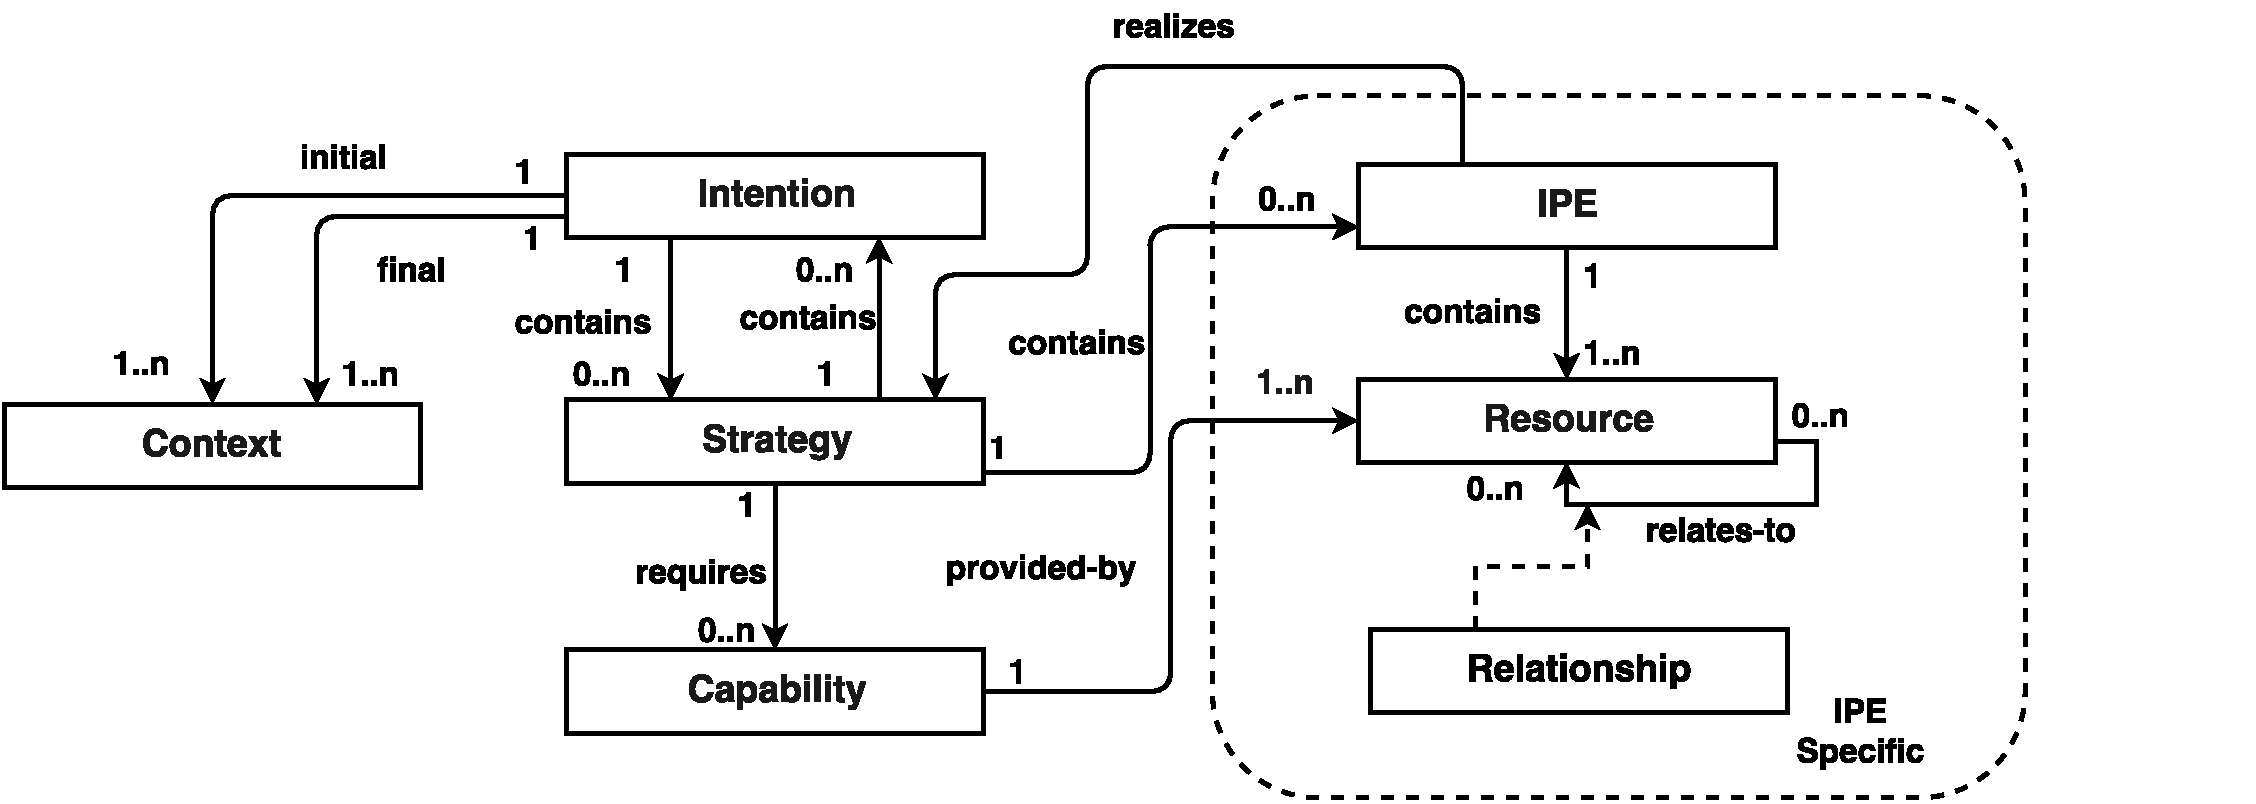
\includegraphics[width=\textwidth]{entity.pdf}
	\caption{Organizational Modeling Entity Types Representation}
	\label{fig:entitymodel}
\end{figure}

In Sungur et al \cite{Sungur2014a} work, the concept of \textit{Informal Process Support Model} (IPSM) has been introduced which is to make use of existing knowledge of human performers. Here the initial creator of the model is experienced human performers. Based on their experience, they add relevant  resources of an informal process. The models are generated at runtime based on the interactions and activities of corresponding human performers. An informal process targets for accomplishment of an intention. The intentions can be refined by defining sub-intentions and/or strategies, which can then be further refined recursively as independent informal processes. The intention-based approach enables describing processes declaratively, i.e., without describing \textit{how} the intention is achieved, and providing only information about \textit{what} is achieved. As the author \cite{Sungur2014a} suggests that this avoids need of predefined business logic in the representations of informal processes. Each resource can be related to another resource in the context of an informal process using predefined or custom \textit{Relationships}. Informal Process Essentials are realized through strategies. Each informal process starts from an initial context, i.e., \textit{initial context} and aims to achieve an intention. After accomplishing the intention, there is a resulting context called as \textit{final context}. The beginning state before achieving intention is called as initial context and the end state after achieving intention is called as final context. On completion of intention execution, the process state changes from one state to another.

%%%%%%%%%%%%%%%%%%%%%%%%%%%%%%%%%%%%%%%%%%%%%%%%%%%%%%%%%%%%%%%%%%%%%%%%%
\section{Overview of Informal Process Essentials}
\label{sec:basicconcepts}
%%%%%%%%%%%%%%%%%%%%%%%%%%%%%%%%%%%%%%%%%%%%%%%%%%%%%%%%%%%%%%%%%%%%%%%%%
In this section, we provide an overview about the concepts introduced in the approach Informal Process Essentials (IPE) \cite{Sungur2014a}. Models are used in various fields like manufacturing, scientific, IT, etc. These models are mainly useful in re-using the predefined regular, intelligible and field-tested solutions. Such models has numerous benefits \footnote{http://www.nomagic.com/getting-started/modeling-benefits.html} like performance improvement, reduced cost of operation and design, etc. Besides these processes there are processes which requires participation of human and performance of these processes depend on human knowledge, i.e., they are subject to change and carried out based on experience of previous knowledge. These processes are called \textit{Informal Processes} and they do not have formal structured execution of steps for the enactment of processes. 

The work by Sungur et. al \cite{Sungur2014a} gives a comprehensive account of challenges in defining the business logic of informal processes as below:

\begin{itemize}
	\item The structure of informal processes are not known before enactment of the processes
	\item Results in less flexible and less efficient solutions
	\item The cost of creation of well-defined business logic is too high
\end{itemize}

This thesis work realizes the concept of \textit{resource-centric modeling of informal processes}, specified in the Informal Process Essentials(IPE) approach by Sungur et al \cite{Sungur2014a}.  As mentioned in the Section \ref{sec:termdefinitions}, resources are drivers to achieve intentions in the informal processes. In this approach author states that, when the desired process result is repeated the same set of resources can be selected and engaged towards collective intention of the informal processes. Also it has been mentioned that each IPE model contains the list of necessary resources to accomplish the main intention of the respective informal process.

In IPE approach, the author differentiates the resources based on the time. The resources that are needed in the informal processes are below :
  \begin{itemize}
  	\item \textit{Initial resources} which are required during the start of informal processes.
  	\item \textit{On-demand resources} that are required based on intentions during process enactment.
  	\item \textit{Actors} are the resources in IPE meta-model, that drive process execution autonomously.
  	\item \textit{Knowledge resources} resources that contain important information required for the enactment of a process. These are critical for guiding actors.  
  \end{itemize}
 
It has been mentioned in the approach \cite{Sungur2014} that Informal Process Essentials (IPE) describes the following about informal process, 1. Describes the constituents informal process such as performers, data and software tools 2. Describes how to make core element ready for the enactment of the informal process i.e resource providers. Predefining business logic would results in higher cost compared to making decisions by human performers during enactment \cite{Sungur2014}. Sometimes, a process team may require participation of  new resources with different roles and relationships from a different team \cite{Matthews2011,Matthews2012}. For example, in our motivating scenario we have two teams  software development team and help desk team. To improve the user feedback portal, help desk team may require resources from software development team with a role of user interface web developer. Thus to satisfy requirement changes, resources are also changeable during process execution. 

%%%%%%%%%%%%%%%%%%%%%%%%%%%%%%%%%%%%%%%%%%%%%%%%%%%%%%%%%%%%%%%%%%%%%%%%%
\section{Human Centric Process}
\label{sec:humancentric}
%%%%%%%%%%%%%%%%%%%%%%%%%%%%%%%%%%%%%%%%%%%%%%%%%%%%%%%%%%%%%%%%%%%%%%%%%
The role of humans in organizations has been evolving over time. The shift from "personnel" to "human resources" acknowledges the importance of humans as organizational resources. There are incredible number of pressure on today's organizations \footnote{http://www.siop.org/tip/backissues/tipjan98/may.aspx} due to varying dynamic nature of organizations. For example, organizational changes like addition of new organizational alliances, new structures and hierarchies, new ways of assigning work, and a very high rate of changes like changes in the workforce, including employees' priorities, capabilities, and demographic characteristics. Thus it is impossible to do one hundred percent perfect forecasting of dynamically changing activities or processes in an organization.

In order to manage such a dynamic environment, organizations need skilled human resources with previous knowledge of handling unforeseen scenarios. Thus human resources are vital part of any organizations as they have skills of acute future orientation to understand changing organizational environment. Humans in an organizations carry out many important activities. Managers and Human Resource (HR) professionals organizes jobs of each and every human in the organization so that they can effectively perform these jobs. Thus humans in any organization are viewed as resources of the organization which is a contemporary part of Human Resource Management \footnote{http://smallbusiness.chron.com/role-human-resource-management-organizations-21077.html}.

When there are multiple human resources working for a process, then there should be some sort of co-ordination and understanding between the humans which is called \textit{collaboration} at an organizational level. Collaboration exists in every levels of an organization. For example at management levels of an organization, managers and HR professionals work together to assign employees their roles and task in the organization. This helps the employees of the organization to adapt to its environment. In a flexible organization, employees roles and responsiblities changes dynamically based on the requirements and business priorities. Thus the need for network of representations between the human resources which sets up an environment to support collaborative work of business related process has been realized in the work by the author Canko\cite{Canko2015}. The concept of \textit{virtual human representation} is an extension of  actor-concept described in  \textit{Informal Process Essentials} \cite{Sungur2014a}. The developed prototype \textit{Human Resource Representation} in the work by the author Canko\cite{Canko2015} saves the information such as capabilities, roles, responsibilities etc.  as a virtual human web ontology instance which can be re-used in web based environments.

These kind of human representation are highly helpful to organizations with dynamically changing processes. These representations can describe and match resources with their capabilities based on the requirements. As we have mentioned in Chapter \ref{chap:introduction}, in our context of resource-centric modeling humans are also considered as resources and we associate \textit{capabilities} with every resources. Moreover, associating capabilities, with resources is helpful in following situation. There can be a situation where resources producing more accurate results for a processing task are preferred than resources which can produce higher throughput for a processing task. Thus we need to associate capabilities with each resources and need to automate the process of discovering and matching the resources with their capabilities based on their process. 

%%%%%%%%%%%%%%%%%%%%%%%%%%%%%%%%%%%%%%%%%%%%%%%%%%%%%%%%%%%%%%%%%%%%%%%%%
\section{Second Phase of InProcXec}
\label{sec:inproxec}
%%%%%%%%%%%%%%%%%%%%%%%%%%%%%%%%%%%%%%%%%%%%%%%%%%%%%%%%%%%%%%%%%%%%%%%%%
In this section, we present an overview about the \textit{Executing Informal Processes} (InProXec) method, proposed by Sungur et al. \cite{Sungur2015}. Since this thesis work is realizing resource-centric modeling of organizations, the main focus of this section is on the second phase of InProXec which is \textit{Informal Process Modeling}(P2). The method described in Figure \ref{fig:inprocxec_steps}, initializes informal process models in an automated fashion. In the following paragraphs, we present short overview about different phases of the InProXec method which has been decribed in detail in the article \cite{Sungur2015} and with a detailed description about the second phase of the \textit{InProXec} method. 

\begin{figure}
	\centering
	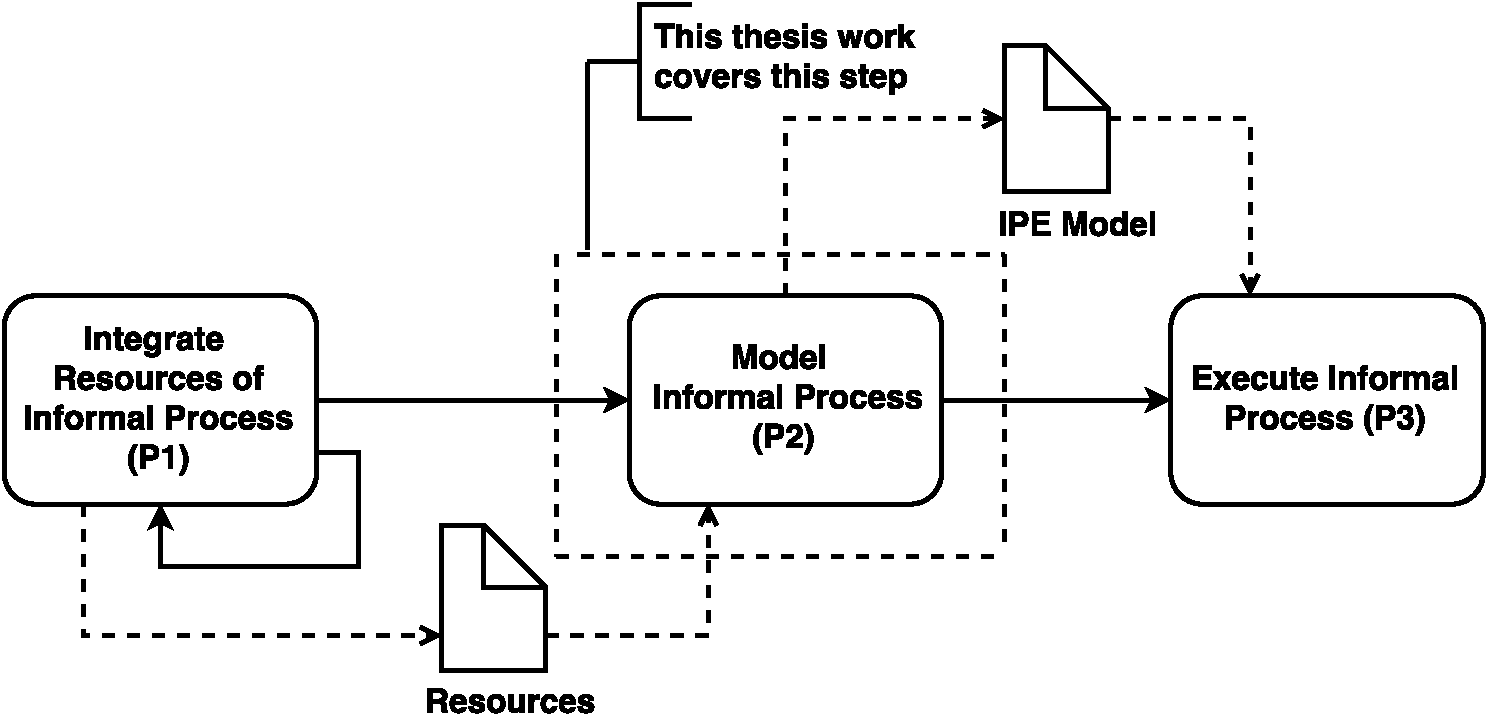
\includegraphics[width= \textwidth]{InProXec_Steps.pdf}
	\caption{Steps of InProXec method \cite{Sungur2015}}
	\label{fig:inprocxec_steps}
\end{figure} 

As shown in the Figure \ref{fig:inprocxec_steps}, the InProcXec method consists of four different phases:

\textit{Integrating Resources of Informal Processes (P1)} - In order to model an informal process, we need information about the resources, these information are collected beforehand during process execution. There exist many services to acquire information about informal processes resources automatically. The final output of this phase is integrated resources which are required as an input to next modeling phase. Thus this phase sets up an environment required for modeling and execution of informal processes.  

\textit{Informal Process Modeling (P2)} - This phase receives the resource definitions made available in the first phase P1 as an input.  Based on this, business experts model informal processes and associated entities like strategies, intentions, capabilities etc., using our developed web editor. This phase has been explained in detail in the following sub section \ref{subsec:informalprocessmodeling}    

\textit{Informal Process Compilation (P3)} - The previous phase P2, describes only the intentions required to be achieved, corresponding required resources etc. But in phase P2, the functionality to instantiate acquirable entities are not included. Thus in third phase P3, the output of phase P2 is taken i.e IPE models and are transformed into intializable self-contained \textit{Deployable Informal Process Essentials Archives(DIPEA)} \cite{Sungur2015} takes place. This results in DIPEAs enacting required informal process. To realize, phase P3 an \textit{IPE Model Compiler} also been introduced. 

\textit{Informal Process Model Deployment and Runtime (P4)} This phase employs \textit{IPE Runtime} which parses DIPEAs and runs the executables contained in those archives. During this phase, the autonomous actors work towards intentions of informal processes using acquired resources and other involved resources.  

%%%%%%%%%%%%%%%%%%%%%%%%%%%%%%%%%%%%%%%%%%%%%%%%%%%%%%%%%%%%%%%%%%%%%%%%%
\subsection{Informal Process Modeling (P2)}
\label{subsec:informalprocessmodeling}
%%%%%%%%%%%%%%%%%%%%%%%%%%%%%%%%%%%%%%%%%%%%%%%%%%%%%%%%%%%%%%%%%%%%%%%%%
This approach of Informal Process Modeling is directed towards modeling the informal process based on their intentions rather than their activities. The developed prototype serves as an holistic web based editor to create, view and update all the associated entities of informal process like intentions, capabilities, strategies etc., along with informal process. Also from our detailed explanation in previous sections about the importance of resources in organizational modeling  and along with the fact that phase P2 receives resource defintions as input from phase P1 of InProXec method we can apprehend that resource definitions are the lowest level in the hierarchy of resource-centric organizational modeling approach. The sequence of steps to be carried out using the developed editor has been shown in the Figure  \ref{fig:processdiagram}. It is important to note that in the figure, only solid round edged rectangles are part of the developed editor. The tasks to be carried out in each of the steps in developed editor is described as below:

\begin{figure}
		\centering
		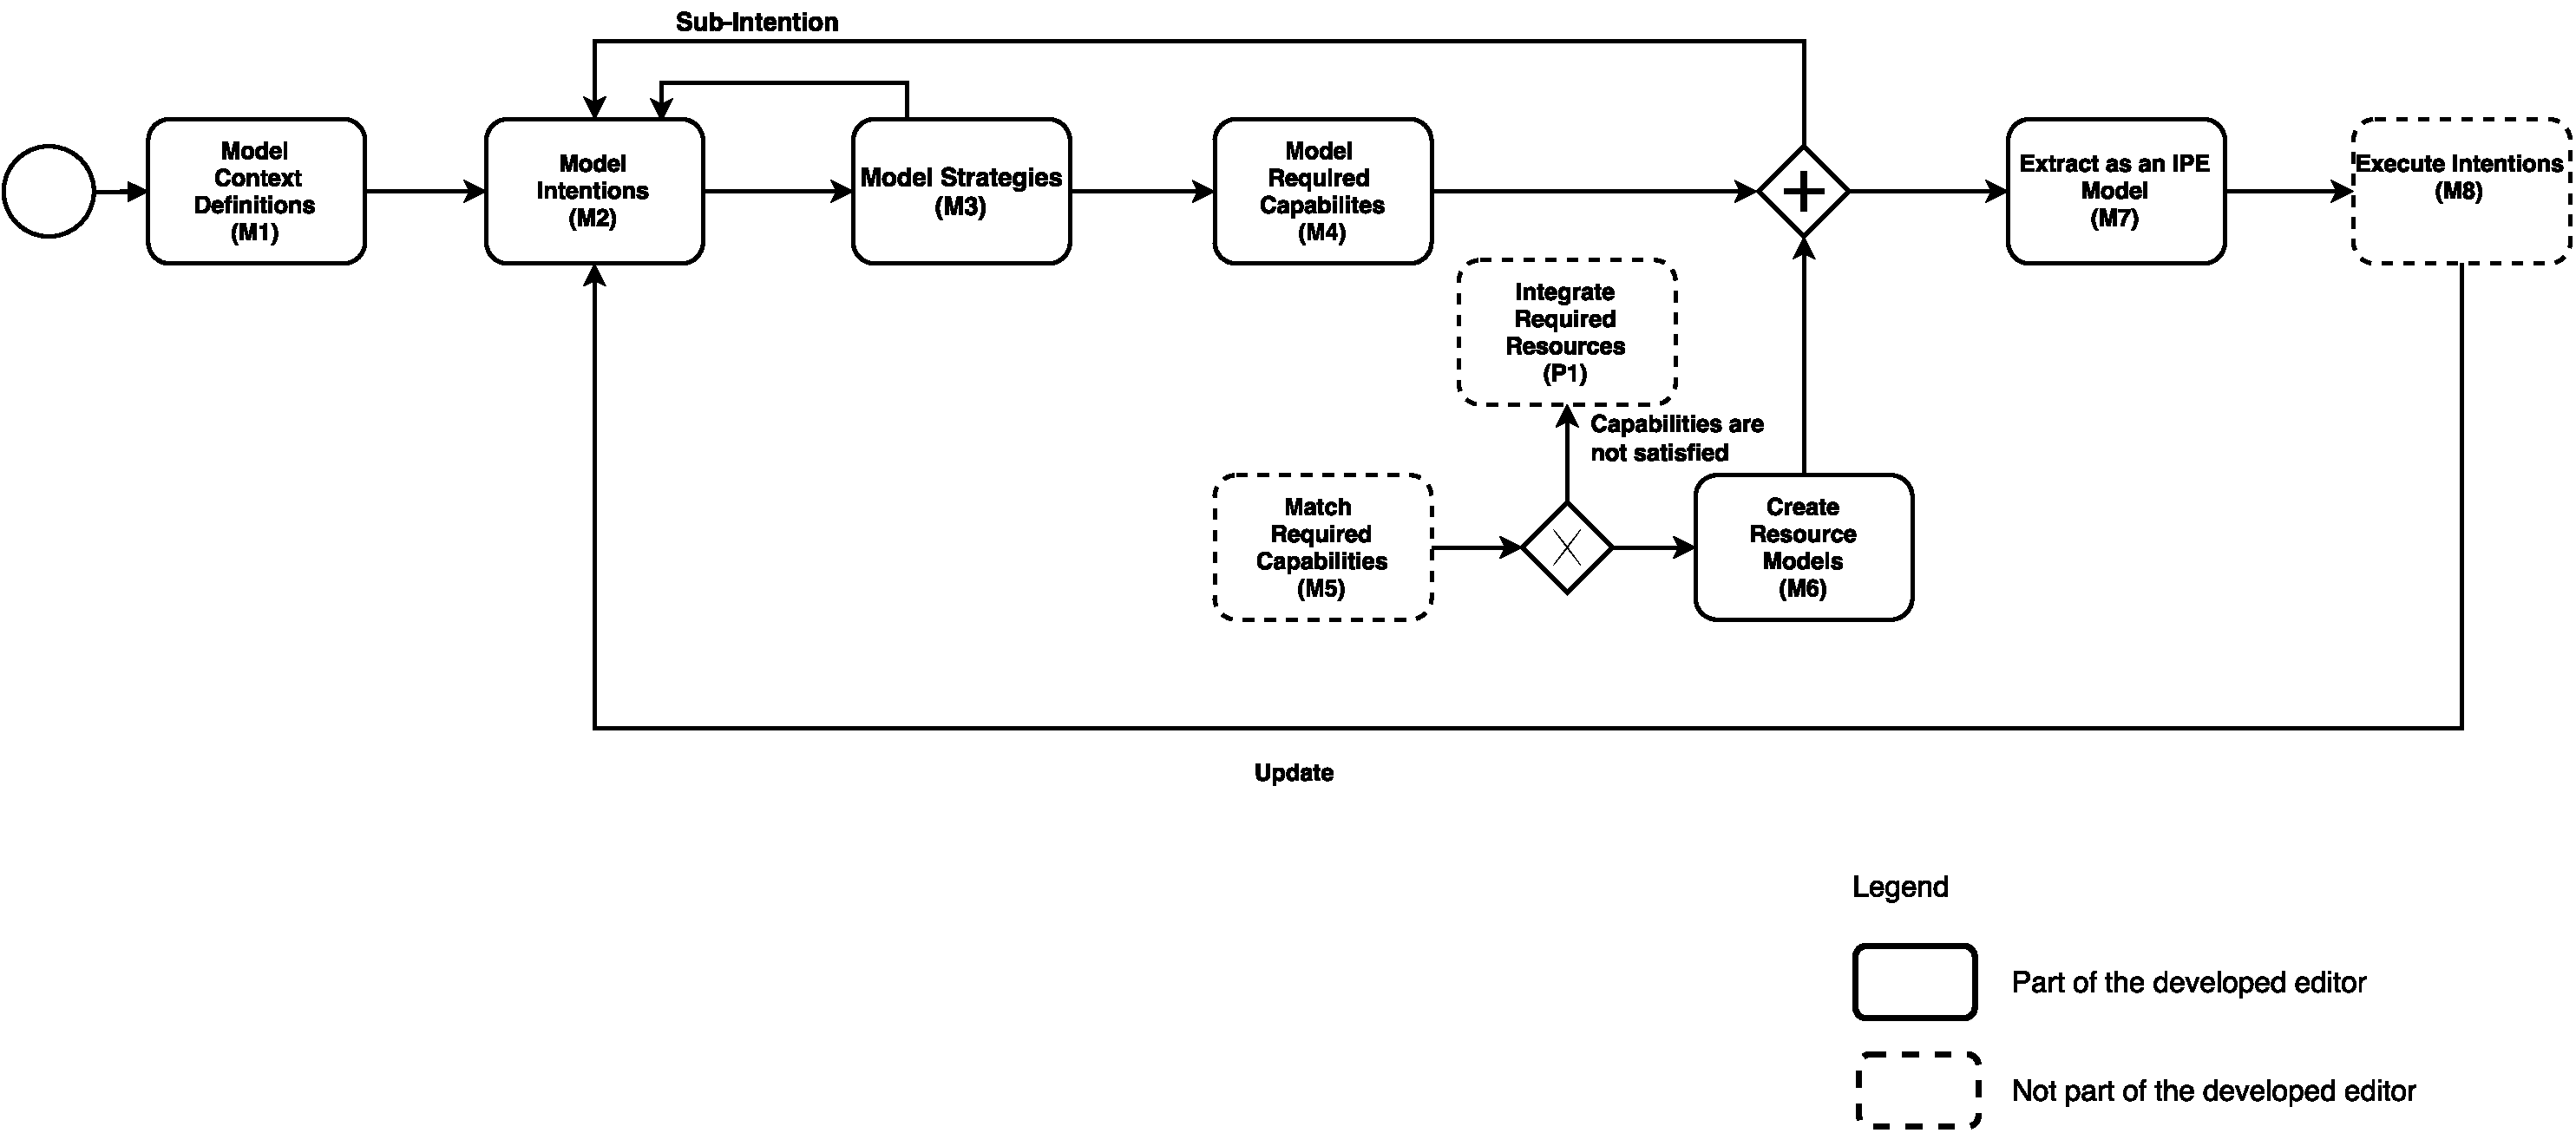
\includegraphics[width=\paperwidth,angle=90]{processmodeling.pdf}
		\caption{Organizational Process Modeling}
		\label{fig:processdiagram}
\end{figure}

\textit{Model Context Definitions} (M1) -  The first step is to model context definitions, where we can model both basic properties like name and namespace of a context definition and entity specific properties like contained contexts, entity definitions etc., of a context definition.  

\textit{Model Intentions} (M2) -  Similar to context definition modeling (M1), the second step (M2) is to model intentions. The context definitions created in step M1 can be used to specify initial and final contexts of an intention. Intentions can contain sub-intentions and contradicting intentions. These type of sub intentions and contradicting intentions are also modeled as intentions in this step and their type of relation to specific intention are mentioned. 

\textit{Model Strategies} (M3) -  Once intentions are identified and modeled, the third step is modeling of strategy to achieve a specific intention. As mentioned earlier in Section \ref{sec:entitytypesrepresentation}, an intention can have multiple strategies. 

\textit{Model Required Capabilities} (M4) - After modeling of strategies, capabilities required to achieve an intention in a specific strategy is modeled. A strategy can require multiple capabilities which has been explained in detail with a suitable example in the following Chapter \ref{chap:motivatingScenario}. 

\textit{Create Resource Models} (M6) -  After matching the resources and capabilities i.e after finding the correct resource that has the capability to carry out the process, the resource models are created. The need for modeling a new intention may arise in parallel this has been explained with a suitable example in the following Chapter \ref{chap:motivatingScenario}.   

\textit{Extract as an IPE Model} (M7) -  After the completion of above mentioned steps, the modeled entities can be extracted as an IPE model which can be reused. 

The other steps denoted in dashed round edged rectangle which are not part of developed web editor includes matching of required organizational capabilities that are satisfied by resource models  to enable the achievement of organizational intentions in certain context definitions through a strategy. If there is no suitable matching capability then phase P1 of InProXec can be carried out again until a matching capability is found. If Capabilites are satisfied resource models can be created. The created resource models(M6) along with modeled capabilities can be extracted as an IPE Model(M7) which will be provided as input for the next step execution of intentions (M8). After the execution of an intention, the status of an intention is updated inside the specific intentions's property. 










